\chapter{Introduction}
\label{ch:introduction}



\section{Introduction}

%\begin{itemize}
%
%    \item What is the subject of the study? Describe the
%        economic/econometric problem.
%
%    \item What is the purpose of the study (working hypothesis)?
%
%    \item What do we already know about the subject (literature
%        review)? Use citations: {\it \citet{Gallant:87} shows that...
%        Alternative Forms of the Wald test are considered
%        \citep{Breusch&Schmidt:88}.}
%
%    \item What is the innovation of the study?
%
%    \item Provide an overview of your results.
%
%
%    \item Outline of the paper:\\
%        {\it The paper is organized as follows. The next section describes %the
%        model under investigation. Section \ref{Sec:Literature Review} %reviews the up-to-date research works.
%        and Section \ref{Sec:Results} presents the results. Finally, %Section
%        \ref{Sec:Conc} concludes.}
%
%    \item The introduction should not be longer than 4 pages.
%
%\end{itemize}




\par The usage of Resource Description Framework \(RDF\) model is recently increasing in diverse fields in computer science, such as Big Data, Machine Learning, Data Science, Data Management, etc. The RDF data model helps computing machines in processing of "meta-data" which is data about data, especially those data about web resources. Moreover, such computing machines will be smarter to understand the data represented in different RDF serialization formats. 

Since the RDF model can facilitate  exchanging of data between software applications and it can be also serialized in multiple formats, such as Turtle\footnote{\href{https://www.w3.org/TR/turtle/}{Turtle}}, N-Triples\footnote{\href{https://www.w3.org/TR/n-triples/}{N-Triples}}, N3\footnote{\href{https://www.w3.org/TeamSubmission/n3/}{N3}}, JSON-LD	\footnote{\href{https://www.w3.org/2018/jsonld-cg-reports/json-ld/}{JSON-LD}}, RDF{/}XML\footnote{\href{https://www.w3.org/TR/rdf-syntax-grammar/}{RDF{/}XML}}, and RDF{/}JSON	\footnote{\href{https://dvcs.w3.org/hg/rdf/raw-file/default/rdf-json/index.html}{RDF{/}JSON}}, then its  quality and correctness needs to be proved before proceeding of any further processing. Most of available  parsers which check for syntax errors in RDF, fail to detect more than one error, especially those represented in Turtle or N-Triples serialization formats. Therefore, there is a need to have more powerful tools that help in listing all such errors or at least most of them.%todo needs to show most used formats  


The motivation of this study is mainly  encouraged by the  tremendous RDF data representation and usage of either Turtle and N-Triples serialization formats in different ontologies and in various sciences, as well as, by the desire to offer a smart solution, capable of listing all or most of syntax errors, particularly, in those two formats. Besides the aim of the study to afford a user-friendly syntax checker of RDF formats, this tool should empower with the ability of recovering some of these syntax errors, essentially, when the errors are common and predefined, such as missing a colon or a dot.  

%TODO need to speak about related work and the outline the result 

The following text in this chapter are divided in a couple of sections to express our motivation of the study, present the problem statement, presents the challenges, list our research contributions, and finally outline how this thesis is structured.  

\subsection{Motivation}

This study was motivated by several software use cases, have as a requirement for their operating, syntax checking of RDF data when it comes as an input. As a motivating example, one of the use cases is discussed in {Figure \ref{Fig:Motivation}}. It describes a collaboration system for processing an input RDF data and let's assume it is performing machine learning classification and analysis. Indeed, in this case, a valid input to the system is required. The input data is initially verified against syntax errors for further data processing, if an error or more are found, the system will stop processing the input data and return a report of errors to the user. The current existing tools (as will be discussed in Chapter \ref{ch:related}) which check the RDF syntax of the input,  only assert that the input is  syntax-error-free. When the input has an error or more, those tools stop  parsing, and further handling, additionally, they report that error to the user. 

Another essential point the abruption of parsing when the first syntax error is found will introduce much complications. Assuming, the input RDF data contains, for example, 10 syntax errors. Normally, what is happening when an error is found, the system will proceed with no further processing, instead it will report the existence of an error, with other information about the error, such an error message, row, and column numbers where the error is occurred. Subsequently, the reported error is commonly corrected by the user to be sent again for re-checking of the syntax. To make it more complex, suppose the user has 10 syntax errors in his RDF input, then, the previous process steps of an input checking, an pause of parsing, an error notifying, and an error correction by the user has to be repeated for 10 times.  Furthermore, when the number of syntax errors increases, the number of error processing and correction processes increases by the same value. Also, imagine what is the consumed time and the work overload to process an input RDF data contains hundreds or thousands of errors.  

	\begin{figure}[ht]
		\begin{center}
			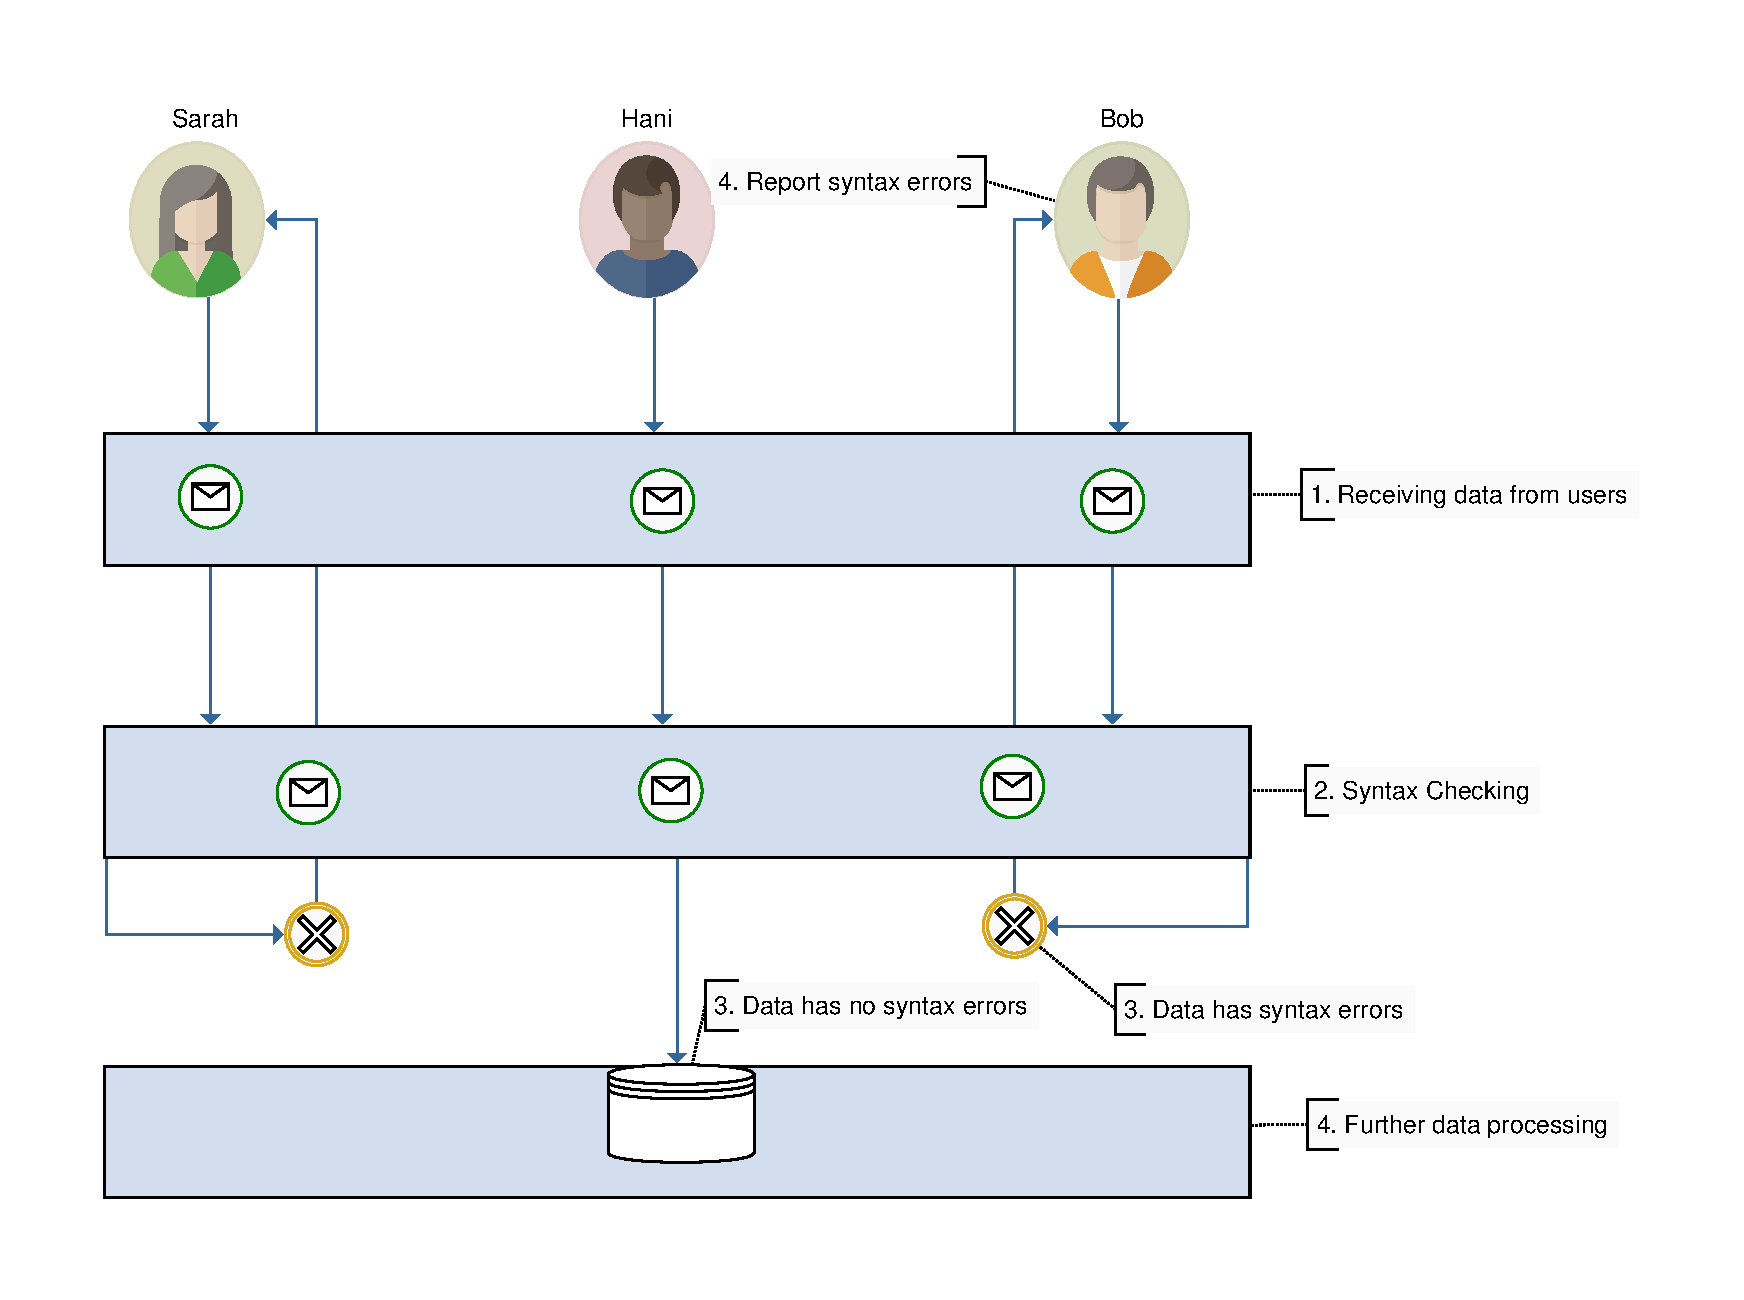
\includegraphics[scale=0.5,angle=0]{images/motivation}
			\caption{\textbf{A motivation example of syntax checking of data before further processing}}
			\label{Fig:Motivation}
		\end{center}
	\end{figure}

let's dig deep in demonstrating what is there in  {Figure \ref{Fig:Motivation}}, It is showing a flow of data from clients or users seeking further data processing. 3 persons are shown in this Figure, their names are Bob, Hani, and Sarah. All of them start with the first phase by sending their data to be syntactically checked. The parser starts checking if there are syntax errors of the input data, if such data passed with no syntax errors, it can be forwarded for further phases, i.e. for data processing, otherwise, the input data will send back to the user to correct the errors. {Figure \ref{Fig:Motivation}} clearly shows that Sarah and Bob have syntax errors in their input data,then, they got an error report, including details about the first detected error. In the meanwhile, Hani has received his data processed without getting such a report, since his input data has no syntax errors. 

This study has been fostered by the former illustrated example to find a suitable solution to allow the parser to continue the whole input of RDF data checking against syntax error and to list them in an error report if any was found. Therefore, the proposed solution focuses on producing a software tool that can detect all syntax errors that can be detected in the input RDF data. 

%\section{Objectives}
\section{Problem Description } 	
The research problem of this study is the unavailability of software tools that can list all the existing syntax errors in RDF files; thus, ontology engineers and users can fix them in one shot. Hence, such a list of errors if it is provided at the end of the syntax checking phase, it significantly assists to get rid of a loop of first error notifications, in case of an existence of multiple errors  in the input data as it was discussed.  

\section{Challenges }
Before reaching the proposed solution, different methods have been tired to reach the objective. The main purpose was the continuation of parsing till the end of the file without stopping on the first syntax error detection  and storing details of the detected errors into a data structure, such as lists. The following 3 tools were individually tested: Jena RIOT API\cite{McBride:2002:JSW:613357.613755}; RDF4J RIO API\cite{RDF4J:Online}; and  N3 Parser\cite{N3Parser:Online}. Both the first and the second are Java\_based RDF tool kit, including a plug-in for RDF parsing, the last is Javascript\_based parser, focused on N-Triple and Turtle serialization formats. In all of these framework, exception handling can be used to catch syntax errors. 

Our task was to remove the text that contains the first detected syntax error from an input text (since those tools fail when the first syntax error is found), then, to supply the remaining text for further parsing. Two methods were used: 1) cutting only the triple or the statement that contains the syntax error, 2) removing text before the found syntax error, including the statement of the error. Both those methods were failed to offer a suitable solution for continuation of parsing after an error discovery, for the following reasons: 1) the difficulty of handling nearby syntax errors, such as errors in the same line or in subsequent statements follow each others, 2) the inexpressive and incomprehensible of error messages, especially, in the second tool, which complicates understanding the actual syntax error for further handling.    


%TODO need references.


\section {Contributions}
In this study, the research work set out to syntactically check RDF data. 
The main contributions of RDF-Doctor (the name of output tool of this study) are:
\begin{enumerate}
	\item  {\bf Listing of detected syntax errors in RDF data:} it is a major goal and contribution where the intention to investigate RDF data, searching for syntax errors. RDF-Doctor is powered by ANTLR framework \cite{ANTLR:Website:Online}, a powerful parser generator, to establish an RDF parser that enables listing of all discovered syntax errors. To elaborate, the basis of the approach is the injection of error production rules inside the grammar which our parser is built based on. Once, the parser detects a combination of tokens from an RDF input that match one of these error production rules, it sends an error notification for an error listener where error lists are stored.
	\item {\bf Reporting syntax errors with user-friendly and expressive messages:} it is of great benefits for debugging and user\_based error corrections when a parser provides user-friendly and meaningful error messages to either normal users or ontology engineer. As the ancient Greek philosopher Socrates said, “Understanding a question is half an answer”\cite{Socrates:quote:Online}, likewise, an understandable error message helps to recover from an error.  RDF-Doctor is not only based on the regular expression input recognition, instead, its recognition is substantially based on grammar rules, each rule represents either a sequence of correct syntax tokens or a sequence of incorrect ones. In case of the latter, RDF-Doctor has a predefined information about each error, hence,  a customized error message can be formulated in an meaningful and convenient way and rendered on-the-fly to the error listener.  
	\item {\bf Automatic error recovery of some syntax errors:} commonly syntax errors in well-know programming languages are those types of missing a dot, adding more dots, or missing semicolon, similarly, happens in RDF data. To limit annoying conflicts while error correction, a certain rule has been set out to control the eligibility of an error to be corrected. The rule is the availability of this error in a predefined error correction list (it includes fundamentally common errors where the action of error recovery of an error is previously known to us), otherwise, it cannot be corrected. For example, on the one hand,  missing of a dot or a semicolon are common mistakes during editing of RDF data, those errors can proficiently correct by RDF-Doctor, but on the other hand, missing of a prefix declaration, decidedly, cannot be corrected since the details of that missing prefix are obscure and unknown.     
\end{enumerate}

\section {Thesis Structure}
The thesis is structured into 7 chapters. Until this spot, \textbf{Chapter \ref{ch:introduction}} was presented, titled with "Introduction". It  includes the general overview of the study, the motivation, the problem description and the challenges, research contributions are also introduced to show how our research work is differed from the state-of-art researches of other scientists. The
remainder of the thesis is organized as follows:
\begin{itemize}
	\item { \textbf{Chapter \ref{ch:preliminaries}:} presents the "Preliminaries" to shed light on the required background to understand what follows in the coming chapters.}
	
	\item {\textbf{Chapter \ref{ch:related}:}} reviews the "Related work" and presents the up-to-date research works. 
		
	\item {\textbf{Chapter \ref{ch:approach}:}} describes the "Approach" of the proposed solution. 
	
	\item {\textbf{Chapter \ref{ch:implementation}:}} demonstrates the "Implementation" of the proposed solution where its architecture and modules are exhibited.
	
	\item {\textbf{Chapter \ref{ch:evaluation}:}} shows the "Evaluation" part where the approach is tested and the results are discussed .

	\item {\textbf{Chapter \ref{ch:conclusions}:}} presents the "Conclusion" to complete this study.
\end{itemize}




%TODO 1- to change the figure in this chapter and improve the caption


